%%=============================================================================
%% Proof of Concept
%%=============================================================================

\chapter{\IfLanguageName{dutch}{Proof of Concept}{Proof of Concept}}
\label{ch:poc}

\section{Inleiding}
\label{poc_inleiding}

In vorige hoofdstukken werd uitgebreid besproken welke vereisten nodig zijn voor een doeltreffende configuratie-inventaris.
Nu is het tijd om deze vereisten in de praktijk te brengen door middel van een Proof of Concept (PoC).
In dit hoofdstuk zal men ons richten op de praktische implementatie van deze vereisten.

Men zal een virtuele-omgeving opzetten, waarbij verschillende gebruikte technologie\"en worden toegelicht die gebruikt zullen worden om de omgeving te automatiseren.
Vervolgens zal men een Bash-script genaamd ConfiScan ontwikkelen, dat dient om de configuratie-inventaris te genereren voor elke server binnen de omgeving.

Tot slot zal men de resultaten van de PoC presenteren.
Hierbij zal men dieper ingaan op de functionaliteit en effectiviteit ervan.
Bovendien is alle bijbehorende code van deze Proof of Concept beschikbaar als open-source, te vinden op GitHub~\autocite{github-poc}.
Dit om de lezer de mogelijkheid te geven om de PoC zelf te testen en te gebruiken, en verder onderzoek mogelijk te maken.

\section{Beperkingen}
\label{poc_beperkingen}

De Proof of Concept (PoC) in deze bachelorproef heeft enkele beperkingen om de scope van het onderzoek te beheersen.
Primair is ervoor gekozen om de PoC te beperken tot enkel het gebruik van Debian als besturingssysteem.
Dit besluit is genomen omdat Debian een veelgebruikte distributie is in de serverwereld, die standaard wordt geleverd met een minimale set aan ge\"installeerde software en configuratie.
Hierdoor biedt het een ideale basis voor het onderzoeken van configuratie-inventaris.

Een andere beperkingen is dat beveiligingsmaatregelen zoals AppArmor en SELinux niet standaard ge\"installeerd zijn op Debian.
Deze zijn dan ook niet aanwezig op de virtuele machines die worden gebruikt voor de PoC.
Dit betekent dat het onderzoek zich voornamelijk zal richten op de standaardconfiguratie van Debian en de inventarisatie van de basisconfiguratie-instellingen.
Hoewel deze beperking de reikwijdte van het onderzoek verkleint, biedt het toch waardevolle inzichten in het proces van configuratie-inventarisatie binnen een specifieke context.

\section{Doelstellingen}
\label{poc_doelstellingen}

Het doel van deze Proof of Concept (PoC) is om een script te ontwikkelen en uit te voeren op de servers, dat de basisconfiguratie verzamelt zoals beschreven in hoofdstuk~\ref{ch:risicoanalyse}, en deze op één centrale locatie plaatst.
Het script zal worden ontworpen om de verschillende eigenschappen van de servers te verzamelen, waaronder netwerkconfiguraties, gebruikers- en groepsinformatie, ge\"installeerde software en andere relevante configuratie-instellingen.

Het is van cruciaal belang dat de verzamelde eigenschappen beschikbaar worden gesteld op een manier die eenvoudig te verwerken is, zoals CSV, JSON en tekstbestanden.
Dit zal het analyseren en verwerken van de verzamelde gegevens vergemakkelijken, en het mogelijk maken om rapporten te genereren en trends te identificeren binnen de configuratie van de servers.
Dit vergemakkelijkt mogelijks verder onderzoek dat kan volgen op deze bachelorproef.

Daarnaast zal het script ook de mogelijkheid moeten bieden om de configuratie van de ge\"installeerde software te kopi\"eren die relevant is voor de rol van de server en deze mee op te slaan in de centrale locatie.
Op deze manier kan men niet alleen de basisconfiguratie van de servers verzamelen, maar ook de specifieke configuratie-instellingen van de software die op elke server is ge\"installeerd.

Het uiteindelijke doel van deze PoC is om een voorbeeld te bieden om op een geautomatiseerde en gestructureerde manier de configuratie van meerdere servers te verzamelen en te beheren.
Door gebruik te maken van een script dat de configuratiegegevens centraliseert en eenvoudig toegankelijk maakt, kan men het beheer en de monitoring van onze serveromgeving verbeteren en effici\"enter maken.

\section{De omgeving}
\label{poc_omgeving}

Om de Proof of Concept uit te voeren, is het noodzakelijk om een virtuele omgeving te cre\"eren die een representatieve setting biedt voor het testen en evalueren van de configuratie-inventaris.
Dit proces omvat verschillende stappen, waaronder het opzetten van virtuele machines, het toewijzen van specifieke rollen aan elke server en het configureren van het netwerk om communicatie tussen de servers mogelijk te maken.

\subsection{Gekozen technologie{\"e}n}
\label{poc_gekozen_technologieen}

Om de omgeving zo reproduceerbaar mogelijk te maken, zal men gebruik maken van verschillende technologie\"en die het opzetten van de omgeving automatiseren.
Dit stelt ons in staat om snel en consistent virtuele machines te cre\"eren en te configureren, wat essentieel is voor een succesvolle uitvoering van de Proof of Concept.

Allereerst zal men gebruik maken van Vagrant~\autocite{vagrant-home}, in combinatie met VirtualBox~\autocite{virtualbox-home}, om de virtuele machines te beheren die de servers zullen vertegenwoordigen binnen deze PoC.
Vagrant biedt een eenvoudige en krachtige manier om virtuele machines te cre\"eren, te provisioneren en te beheren, waardoor men snel en effici\"ent onze testomgeving kunnen opzetten en terug afbreken tijdens het testen van de code.

Daarnaast zal men Ansible~\autocite{ansible-home} gebruiken om elke server individueel te configureren en zijn specifieke rol binnen de omgeving te vervullen.
Ansible is een krachtige IaC-tool die ons in staat stelt om complexe configuratietaken uit te voeren met behulp van eenvoudig te begrijpen YAML-bestanden~\autocite{ansible-docs-yaml}.
Met Ansible kan men de configuratie van elke server nauwkeurig defini\"eren en consistent toepassen, wat bijdraagt aan de betrouwbaarheid en reproduceerbaarheid van onze omgeving.
Dit doordat dit een van de fundamenten is van IaC, zoals besproken in~\ref{sub:iac}.

\subsection{Serverrollen}
\label{poc_serverrollen}

De opgezette omgeving zal bestaan uit zes servers, waarvan vijf servers worden toegewezen aan verschillende serverrollen die men wil inventariseren, en één server zal fungeren als de centrale locatie voor de configuratie-inventaris en als de controller voor de servers.
In dit gedeelte zal men de diverse rollen van de servers bespreken, evenals de gebruikte software om deze rollen te vervullen.

De keuze voor de serverrollen is tot stand gekomen in samenwerking met de co-promotor van deze bachelorproef, en deze rollen vertegenwoordigen een representatieve set van servers die vaak in de praktijk worden ingezet.
Dit zorgt ervoor dat onze PoC een breed scala aan serverconfiguraties kan omvatten en ons in staat stelt om een grondige inventarisatie uit te voeren van de configuratie-instellingen die relevant zijn voor elk type server.

Alvast een overzicht van de verschillende servers die deel zullen uitmaken van de omgeving, samen met de rol is te vinden in tabel~\ref{table:poc-server-roles}.

\begin{table}[!h]
    \begin{center}
        \begin{tabular}{ c c c }
            \hline
                Servernaam & IP-adres & Rol \\ [0.5ex]
            \hline
            control & 172.16.128.253 & Ansible-controller \\
            srv1    & 172.16.128.1   & DNS-server \\
            srv2    & 172.16.128.2   & Webserver \\
            srv3    & 172.16.128.3   & Database-server \\
            srv4    & 172.16.128.4   & Monitoring-server \\
            srv5    & 172.16.128.5   & Fileserver \\
        \end{tabular}
    \end{center}
    \caption[Rollen toegewezen aan servers.]{Overzicht van de verschillende rollen die worden toegewezen aan elke server binnen de omgeving.}
    \label{table:poc-server-roles}
\end{table}


\subsubsection{Ansible-controller}
\label{poc_ansible_controller}

De server met de naam \texttt{control} heeft de rol om de configuratie van de andere servers binnen de omgeving te beheren met behulp van Ansible.
Men zal deze server gebruiken om via Ansible het Bash-script uit te voeren op elke server.
Dit stelt ons in staat om de nodige bestanden met betrekking tot de configuratie-inventaris te verzamelen en te centraliseren op \'e\'en locatie.

\subsubsection{DNS-server}
\label{poc_dns_server}

De eerste server zal de rol van DNS-server binnen de omgeving vervullen.
Hiervoor zal men gebruikmaken van de BIND DNS-server~\autocite{bind-home}, een van de meest gebruikte DNS-servers in de serverwereld.

Deze server zal een DNS-zone bevatten voor het domein \texttt{poc.lan}, waarbij de server zelf fungeert als de primaire nameserver voor deze zone.\
Hierdoor zal het gecentraliseerde DNS-informatie bevatten voor de andere servers binnen de omgeving, zoals IP-adressen en hostnamen.
Dit stelt ons in staat om de servers te bereiken via hun fully-qualified domain name (FQDN), in plaats van alleen hun IP-adres.
Bijvoorbeeld, kan men \texttt{srv1.poc.lan} gebruiken om de eerste server te bereiken, in plaats van \texttt{172.16.128.1}, dat het IP-adres van de DNS-server zelf zou zijn.

Wanneer een DNS-query niet kan worden beantwoord door de DNS-server zelf, zal deze worden doorgestuurd naar de DNS-server van de ISP.
Dit wordt mogelijk gemaakt door gebruik te maken van de NAT-interface van VirtualBox, waarbij Google (\texttt{8.8.8.8}) of Cloudflare (\texttt{1.1.1.1}) als backup DNS-servers zullen fungeren.

\subsubsection{Webserver}
\label{poc_webserver}

De tweede server, met hostname \texttt{srv2}, zal de rol van webserver vervullen binnen de omgeving.
Men heeft ervoor gekozen om een basis Apache-webserver~\autocite{apache-home} te installeren, die een geconfigureerde website zal tonen wanneer deze wordt bezocht via een webbrowser.
De website zal bestaan uit een eenvoudige PHP-pagina die de inhoud van de database, geconfigureerd op \texttt{srv3}, zal weergeven.

\subsubsection{Database-server}
\label{poc_database_server}

Op \texttt{srv3} wordt een MariaDB-databaseserver~\autocite{maria-home} ge\"installeerd, die een database zal hosten met meerdere tabellen en records.
Deze tabellen zullen worden aangemaakt en gevuld met gegevens door gebruik te maken van een SQL-script, ontwikkeld door Patrick Allaert en openbaar beschikbaar op GitHub~\autocite{github-sql-script}.

De server zal verkeer van alle hosts binnen het netwerk toestaan en zal een specifieke gebruiker genaamd \texttt{appuser} bevatten.
Deze gebruiker heeft toegang tot de database, genaamd \texttt{appdb}, en de bijbehorende tabellen.

\subsubsection{Monitoring-server}
\label{poc_monitoring_server}

De vierde server, met de naam \texttt{srv4}, zal de rol van monitoring-server vervullen binnen de omgeving.
Hierop wordt Prometheus~\autocite{prometheus-home} ge\"installeerd, een veelgebruikte monitoringtool die wordt ingezet om metrische gegevens te verzamelen en te visualiseren van diverse systemen en services.
Deze server wordt geconfigureerd om alle metrische gegevens van de andere servers binnen de omgeving te verzamelen en te presenteren.

Dit wordt mogelijk gemaakt door het installeren van Node Exporter~\autocite{node-exporter-home} op elke server.
Node Exporter exposeert de metrische gegevens van de servers aan Prometheus, waardoor deze gegevens kunnen worden verzameld en geanalyseerd.

\subsubsection{Fileserver}
\label{poc_fileserver}

De laatste server die een specifieke rol zal vervullen binnen de omgeving is de fileserver, met de naam \texttt{srv5}.
Op deze server wordt een Samba-fileserver~\autocite{samba-home} ge\"installeerd.
Deze Samba-server biedt een gedeelde directory aan, specifiek genaamd \texttt{/mnt/storage\_01}, die beschikbaar is voor de andere servers binnen de omgeving.

Bovendien wordt er een gebruiker genaamd \texttt{james} aangemaakt, die lid is van de \texttt{sudo}-groep.
Deze gebruiker krijgt toegang tot de Samba-share en kan bestanden zowel lezen als schrijven naar deze share.

Daarnaast wordt voor de gebruiker een specifieke \texttt{sudo}-regel ingesteld, waardoor hij het \texttt{apt}-commando kan uitvoeren zonder een wachtwoord in te voeren.

\section{Ontwerp en implementatie}
\label{poc_ontwerp_implementatie}

In dit gedeelte zullen enkele ontwerp keuzes worden besproken die zijn gemaakt tijdens de ontwikkeling van het script, en hoe deze keuzes hebben bijgedragen aan de functionaliteit en effectiviteit van de Proof of Concept.
Voor een gedetailleerd overzicht van hoe de Proof of Concept werd uitgevoerd op elke server, verwijst men naar bijlage~\ref{ch:bijlage_poc_uitvoering}.

\subsection{Bourne Again Shell (Bash)}
\label{poc_bash}

De Bourne Again Shell (Bash)~\autocite{gnu-bash-home} is een veelgebruikte shell, ook wel command language interpreter genoemd, die oorspronkelijk is ontwikkeld door de Free Software Foundation onder het GNU-project.
Aanvankelijk bedacht als een krachtiger alternatief voor de standaard Bourne Shell (sh) op GNU/Linux-systemen, heeft Bash zich ontwikkeld tot een van de meest populaire shells in de Linux-wereld.
Het wordt vaak gebruikt voor het schrijven van scripts en het automatiseren van diverse taken.

Een van de sterke punten van Bash is de hoge mate van compatibiliteit met zijn voorganger, de Bourne Shell, terwijl het ook handige functies uit andere shells zoals de Korn Shell (ksh) en de C Shell (csh) heeft ge\"integreerd.

De veelzijdigheid van Bash maakt het een uitstekende keuze voor het schrijven van scripts die verschillende taken moeten uitvoeren, zoals het verzamelen van configuratiegegevens van een server.
In combinatie met andere krachtige tools zoals \texttt{awk} en \texttt{sed}, kan Bash worden gebruikt om specifieke gegevens uit bestanden te filteren, te verwerken en op een leesbare manier weer te geven, alsook het automatiseren van verschillende taken.

\subsection{Comma-Separated Values (CSV)}
\label{poc_functionaliteiten_csv}

Een van de doelstellingen is om de configuratie-informatie op een zo toegankelijk mogelijke manier weer te geven.
Daarom is ervoor gekozen om veel van deze configuratie-eigenschappen te presenteren in CSV-formaat, ook wel bekend als Comma-Separated Values.
Dit tekstformaat maakt het mogelijk om gegevens in tabelvorm weer te geven, waarbij elke rij een record vertegenwoordigt en de kolommen de eigenschappen van dat record bevatten.
De gegevens worden gescheiden door komma's en elke nieuwe regel markeert een nieuwe rij.
CSV is een veelgebruikt formaat dat is ontworpen voor het importeren en exporteren van gegevens tussen verschillende programma's~\autocite{shafranovich2005common}.

Een voorbeeld van het gebruik van dit formaat is bij het overbrengen van gegevens van een databank naar een spreadsheetprogramma zoals Microsoft Excel.
De meeste spreadsheetprogramma's kunnen CSV-bestanden importeren en exporteren~\autocite{shafranovich2005common}.
Dit maakt het eenvoudig om basisconfiguratie, zoals netwerkinterfaces van een server, over te zetten naar een spreadsheetprogramma.

Daarnaast zullen ook gewone tekstbestanden worden gebruikt om gegevens op te slaan.
Dit is vooral het geval voor complexe informatie waarvoor CSV niet geschikt is en het gebruik van CSV de leesbaarheid zou verminderen.
Een voorbeeld hiervan zijn de firewallregels, die vaak complexe configuraties bevatten en beter kunnen worden weergegeven in een tekstbestand.
Het weergeven van deze informatie in CSV-formaat zou de leesbaarheid van de gegevens verminderen, wat men zoveel mogelijk willen vermijden.

\begin{listing}
  \begin{minted}[linenos,tabsize=4,breaklines]{console}
Unit,State,Preset
cups.path,enabled,enabled
abrt-journal-core.service,enabled,enabled
abrt-oops.service,enabled,enabled
abrt-vmcore.service,enabled,enabled
abrt-xorg.service,enabled,enabled
abrtd.service,enabled,enabled
accounts-daemon.service,enabled,enabled
akmods.service,enabled,enabled
auditd.service,enabled,enabled
avahi-daemon.service,enabled,enabled
[...]
  \end{minted}
  \caption[Enabled systemd units in CSV-formaat.]{Voorbeeld van alle enabled systemd units op een server in CSV-formaat.}
  \label{lst:poc-network-csv}
\end{listing}

\subsection{Applicatie specifieke configuratie}
\label{poc_functionaliteiten_app_config}

Het script biedt ook een flexibele manier om de configuratie van specifieke applicaties op de servers te inventariseren, zoals vereist in de doelstellingen.
Voor deze bachelorproef is ervoor gekozen om de gebruiker zelf de configuratiebestanden of directories te laten kiezen en specificeren als argumenten bij het uitvoeren van het script.
Deze aanpak geeft de gebruiker de vrijheid om de configuratie van specifieke applicaties te selecteren die relevant zijn voor hun behoeften en omgeving.
Wanneer men geen specifieke configuratiebestanden of directories opgeeft, zal het script een kopie maken van de gehele \texttt{/etc}-directory, die de meeste configuratiebestanden bevat voor de ge\"installeerde software op de server.

Wanneer het script wordt uitgevoerd, kunnen gebruikers eenvoudig de gewenste configuratiebestanden of -directories opgeven als argumenten.
Zoals te zien is in listing~\ref{lst:poc-config-args}, wordt het script uitgevoerd met de configuratiebestanden van Apache en de SSH-daemon als argumenten.

\begin{listing}
  \begin{minted}[linenos,tabsize=4,breaklines]{console}
vagrant@srv1:~$ ./confiscan.sh /etc/apache2/apache2.conf /etc/ssh/sshd_config
  \end{minted}
  \caption[Uitvoeren van script met configuratiebestanden.]{Voorbeeld van het uitvoeren van het script met specifieke configuratiebestanden als argumenten.}
  \label{lst:poc-config-args}
\end{listing}

\subsection{/proc-bestandssysteem}
\label{poc_functionaliteiten_proc}

Het \texttt{/proc}-bestandssysteem is een virtueel bestandssysteem dat kan worden beschouwd als een schat aan informatie over het systeem.
Het is een speciaal bestandssysteem dat Linux heeft ge\"erfd van zijn voorganger, UNIX, en dat een breed scala aan informatie bevat over de actieve processen, kernelmodules, hardwareconfiguratie en andere systeemgerelateerde gegevens.
Beheerd door de Linux-kernel zelf en vaak read-only voor reguliere gebruikers, kan het worden beschouwd als een bron van waarheid voor informatie over het systeem~\autocite{rhel-proc}.

\begin{listing}
  \begin{minted}[linenos,tabsize=4,breaklines]{console}
[anton@fedorable ~]$ cat /proc/sys/kernel/hostname
fedorable
  \end{minted}
  \caption[Weergave van server hostname.]{Voorbeeld van het weergeven van de hostname van de server.}
  \label{lst:poc-proc-hostname}
\end{listing}

Enkele handige bestanden binnen het \texttt{/proc}-bestandssysteem zijn, die ook zullen worden gebruikt in het script, zijn:

\begin{itemize}
    \item \texttt{/proc/sys/kernel/hostname}: Bevat de hostname van de server, zoals weer te geven in listing~\ref{lst:poc-proc-hostname}.
    \item \texttt{/proc/cmdline}: Bevat de boot parameters die zijn doorgegeven aan de kernel tijdens het opstarten.
    \item \texttt{/proc/modules}: Lijst van alle geladen kernel modules.
    \item \texttt{/proc/filesystems}: Lijst van alle bestandssystemen die door de kernel worden ondersteund.
    \item \texttt{/proc/mounts}: Lijst van alle actieve mount points op het systeem.
\end{itemize}

Tijdens deze Proof of Concept zal men naast het verwerken van commando's ook informatie verzamelen uit dit virtuele bestandssysteem.
Men zal gegevens verzamelen over kernelmodules, actieve mount points en andere systeemgerelateerde informatie.
Vervolgens zal men deze informatie verwerken en opslaan in de configu-\ ratie-inventaris in een leesbare vorm, zoals CSV- of tekstbestanden.

\section{De resultaten}
\label{poc_resultaten}

Tijdens de ontwikkelingsfase van het script werd er rekening gehouden met de besproken onderwerpen uit hoofdstuk~\ref{ch:risicoanalyse}.
Hierdoor is men erin geslaagd om een script te ontwikkelen dat de configuratie-inventaris van een server kan genereren.
Na het uitvoeren van het script op elke server binnen de omgeving, heeft men voor elke server een directory met bestanden ontvangen die verschillende eigenschappen van de server bevatten.
Als de \texttt{-t} optie wordt gebruikt, wordt er een tarball gegenereerd van deze directory.
Dit maakte het eenvoudig om de configuratie-inventaris te verzamelen en te centraliseren op de controller-server, waar men de gegevens kunnen analyseren en verwerken.
Tabel~\ref{table:poc-inventory-properties} toont een algemeen overzicht van de eigenschappen die al dan niet zijn opgenomen in de configuratie-inventaris.

Uit de resultaten vermeld in tabel~\ref{table:poc-inventory-properties} kan men concluderen dat de meeste eigenschappen van de serverconfiguratie met succes zijn opgenomen in de configuratie-inventaris.
Echter zijn er enkele beperkingen, waaronder het ontbreken van de AppArmor- en SELinux-configuraties, die niet zijn opgenomen in de configuratie-inventaris.
Dit kan worden opgelost door de directory of configuratiebestanden van deze beveiligingsmaatregelen mee te geven als commandline-argumenten.
Dit zorgt ervoor dat de configuratiebestanden toch worden opgenomen in de confi-\ guratie-inventaris.

Een alternatieve aanpak is het toevoegen van een aparte sectie waarin men de configuratie van AppArmor en SELinux kunnen opnemen.
Indien gewenst kunnen deze gegevens dan worden omgezet naar een leesbaar formaat, zoals CSV of tekstbestanden.
Echter is ervoor gekozen om dit specifieke aspect niet in deze bachelorproef op te nemen, zowel om de scope te beperken als omdat Debian standaard geen AppArmor of SELinux ge\"installeerd heeft.

Een andere beperking heeft betrekking op het opnemen van specifieke softwareconfiguraties.
Wanneer een directory of bestand wordt meegegeven als argument, wordt dit letterlijk gekopieerd naar de configuratie-inventaris.
Dit houdt geen rekening met het soort bestand.
Als het bijvoorbeeld een softlink is, bestaat de kans dat deze niet zal werken na het inventariseren van de configuratie.
Dit werd vastgesteld tijdens het testen van het script op \texttt{srv2}, waar men de \texttt{my.cnf} van MariaDB wilden opnemen in de configuratie-inventaris.
Maar dit een softlink was naar \texttt{/etc/alternatives/my.cnf}, wat niet werd meegegeven als argument.

Wanneer het echter een softlink betreft naar een bestand binnen de gespecificeerde directory, zal deze wel blijven werken.
Dit werd bevestigd na het uitvoeren van het script op \texttt{srv3}, waarbij men succesvol de configuratie van Apache, inclusief de softlinks van de modules in \texttt{/etc/apache2/mods-enabled}, hebben opgenomen in de configuratie-inventaris.

\def\checkmark{\tikz\fill[scale=0.4](0,.35) -- (.25,0) -- (1,.7) -- (.25,.15) -- cycle;}
\begin{table}[!h]
    \begin{center}
        \begin{tabular}{ c c c }
            \hline
                Eigenschap & Opgenomen & Niet opgenomen \\ [0.5ex]
            \hline
                AppArmor                        &            & \checkmark \\
                BIOS-informatie                 & \checkmark &            \\
                Bestandssystemen                & \checkmark &            \\
                Besturingssysteem               & \checkmark &            \\
                Boot parameters                 & \checkmark &            \\
                CPU-informatie                  & \checkmark &            \\
                Cronjobs                        & \checkmark &            \\
                DNS-configuratie                & \checkmark &            \\
                Firewallregels                  & \checkmark &            \\
                Ge\"installeerde software       & \checkmark &            \\
                Gebruikers                      & \checkmark &            \\
                Geheugeninformatie              & \checkmark &            \\
                Groepen                         & \checkmark &            \\
                Kernelmodules                   & \checkmark &            \\
                Kernelversie                    & \checkmark &            \\
                Mount points                    & \checkmark &            \\
                Netwerkinterfaces               & \checkmark &            \\
                Partities                       & \checkmark &            \\
                Repositories                    & \checkmark &            \\
                Routingtabel                    & \checkmark &            \\
                SELinux                         &            & \checkmark \\
                Specifieke softwareconfiguratie & \checkmark &            \\
                Systeeminformatie               & \checkmark &            \\
                Systemd units                   & \checkmark &            \\
                TCP/UDP-poorten                 & \checkmark &            \\
                \text{sudo}-regels              & \checkmark &            \\
        \end{tabular}
    \end{center}
    \caption[Eigenschappen in configuratie-inventaris.]{Overzicht van de eigenschappen die al dan niet zijn opgenomen in de configuratie-inventaris.}
    \label{table:poc-inventory-properties}
\end{table}

De resultaten van het script zijn systematisch vergeleken met zowel de configuratie die door Ansible is toegepast op de servers als de daadwerkelijke configuratie van de servers zelf.
Aangezien het script de configuratie van de applicaties reproduceert, komen deze gegevens in de configuratie-inventaris overeen met de configuratie die door Ansible is toegepast.
Het implementeren van een file-integriteitscon-\ trole, zoals gedaan door het script met behulp van \texttt{sha256sum}, kan een extra laag van controle bieden om de integriteit van de configuratiebestanden te waarborgen.
Bovendien stelt het ons in staat om later eventuele wijzigingen in de configuratiebestanden te identificeren.
Wanneer men de resultaten van de configuratie die door Vagrant doorgevoerd werd bekijken, merkt men op dat deze ook overeenkomen met de specificaties in het \texttt{vagrant-hosts.yml} bestand.
Deze resultaten betreffen voornamelijk de netwerkconfiguratie, zoals IP-adressen en hostnamen.

Over het algemeen biedt het script een solide basis voor verdere ontwikkeling en uitbreiding van de configuratie-inventaris met meer eigenschappen en functionaliteiten op Debian-servers.
Bijna elke beperking die tijdens het testen van het script is ge\"identificeerd, kan worden overwonnen door de functionaliteit van het script uit te breiden en te verbeteren.
Een mogelijke oplossing voor het probleem met softlinks is bijvoorbeeld het implementeren van een mechanisme dat de bestanden volgt en controleert of het al dan niet een link is.
Als het een link is, kan het script de link volgen en het gekoppelde bestand ook toevoegen aan de configuratie-inventaris.
Een alternatieve oplossing, waarbij gebruik wordt gemaakt van \texttt{rsync}, wordt behandeld in bijlage~\ref{ch:bijlage_symlink_kopieren_met_rsync}.

Bovendien kan men door het gebruik van bestandsformaten zoals CSV en tekstbestanden de verkregen resultaten eenvoudig visualiseren.
Dit kan worden gedaan met behulp van spreadsheetprogramma's of door het ontwikkelen van aangepaste applicaties voor verder onderzoek en analyse.
Een voorbeeld hiervan is te zien in figuur~\ref{fig:mountpoints-csv-import-spreadsheet}, waar de mount points van \texttt{srv1} zijn ge\"importeerd in OnlyOffice, een documentverwerker die spreadsheetfunctionaliteit biedt.

\begin{figure}[h!]
    \begin{center}
        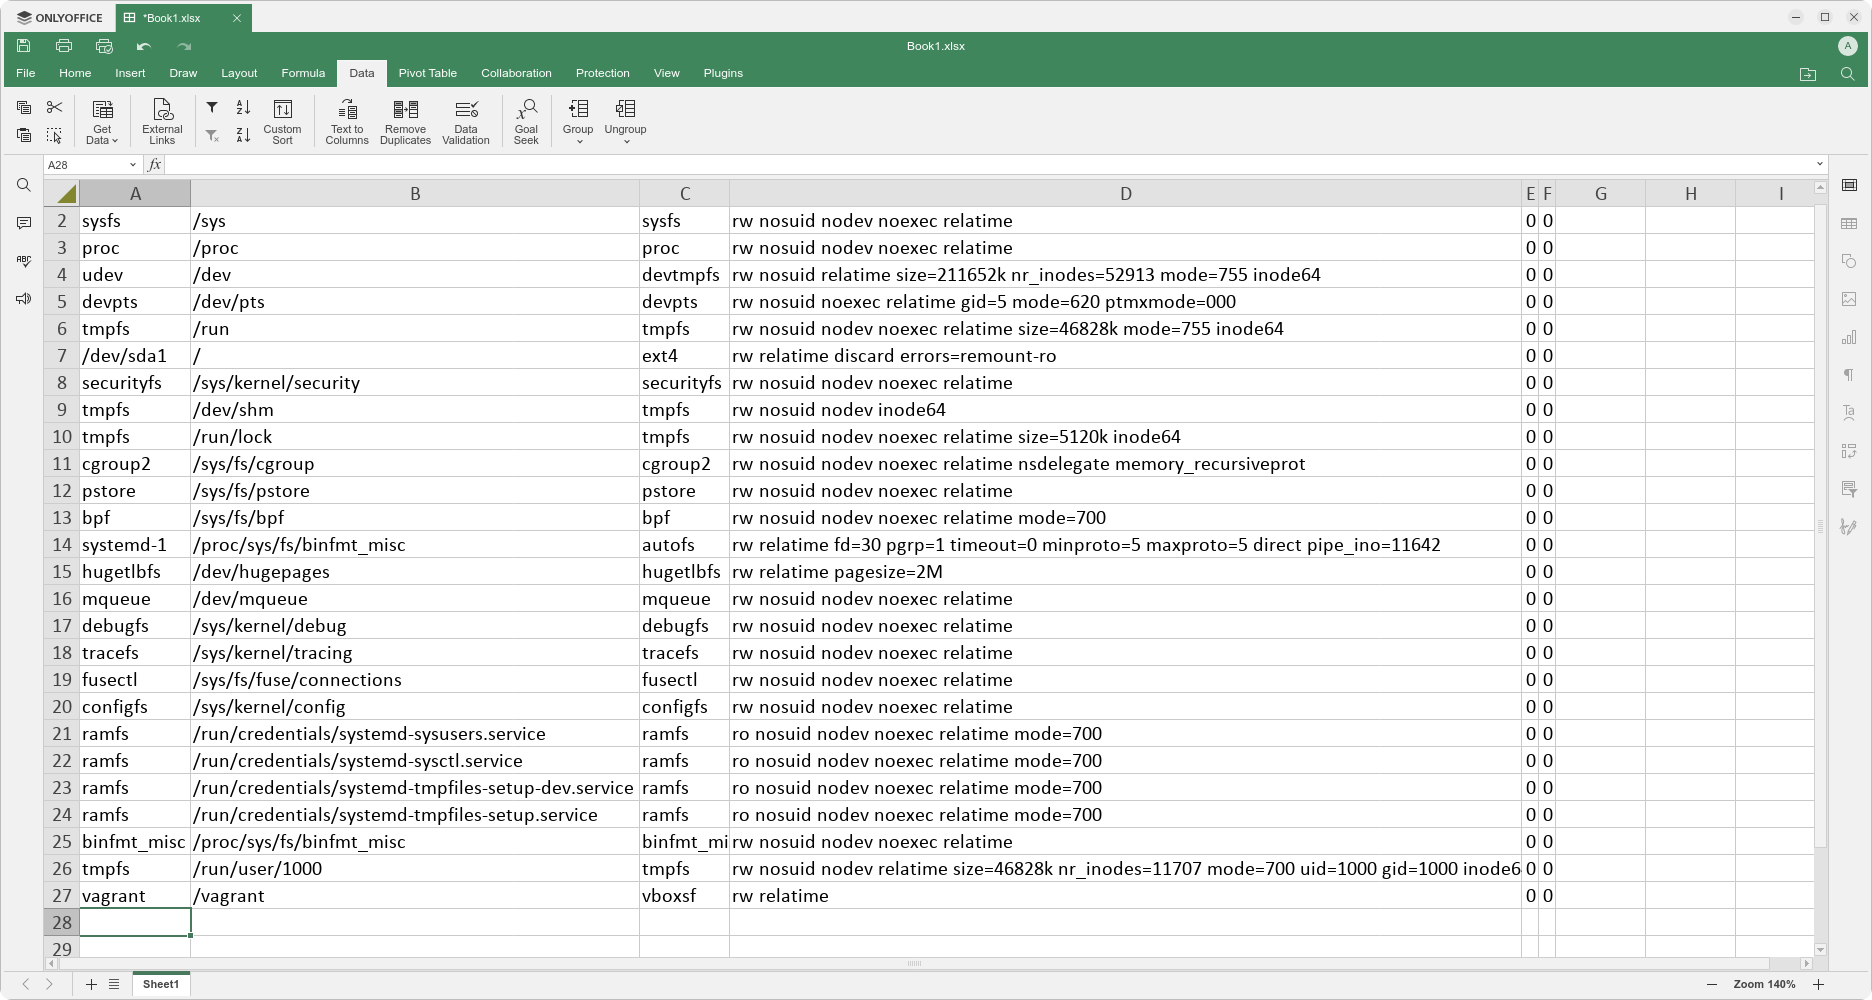
\includegraphics[width=\textwidth]
        {./graphics/mountpoints-csv-import-spreadsheet.png}
        \caption[Voorbeeld van mount points in spreadsheet.]{\label{fig:mountpoints-csv-import-spreadsheet}Voorbeeld van de mount points van \texttt{srv1} ge\"importeerd in een spreadsheetprogramma.}
    \end{center}
\end{figure}

Een voorbeeld van de uitvoer van het script is te vinden in bijlage~\ref{ch:bijlage_confiscan}.

\section{Toekomstig onderzoek}
\label{poc_toekomstig_onderzoek}

Tijdens de PoC lag de nadruk vooral op het verzamelen van configuratie-informatie van Debian-servers.
Een mogelijke uitbreiding van dit onderzoek zou het toevoegen van compatibiliteit met andere distributies omvatten, zoals Red Hat Enterprise Linux (RHEL), Oracle Linux of AlmaLinux.
Deze distributies worden vaak gebruikt in productieomgevingen en hebben andere configuraties dan een standaard Debian installatie.

Naast het toevoegen van compatibiliteit met andere distributies, kan het ook interessant zijn om de functionaliteit uit te breiden naar cloudomgevingen.
Hiervoor zou men API-calls kunnen gebruiken om de configuratie te verzamelen.
Dit zou niet alleen inzicht geven in de serverconfiguraties, maar ook in de infrastructuur waarin ze zich bevinden.

Een andere waardevolle toevoeging aan het script zou zijn om specifieke code toe te voegen voor het verzamelen van AppArmor- en SELinux-configuraties.
Hierdoor wordt het script completer en kan een breder scala aan configuratie-instellingen worden ge\"inventariseerd, zonder dat de eindgebruiker deze configuratiebestanden als argumenten moet opgeven tijdens de uitvoering.

In de PoC werd gebruik gemaakt van Ansible om het script op elke server uit te voeren.
Aangezien het doel is om aan de hand van de verzamelde configuratie-inventaris een beeld te krijgen van de configuratie en over te schakelen naar een IaC-omgeving, zou het waardevol zijn om het script te voorzien van een mechanisme om zelf verbinding te maken met de servers en het vervolgens uit te voeren.
Dit zou kunnen worden bereikt door een wrapper script te schrijven dat het script uploadt naar elke server via \texttt{scp} en het vervolgens uitvoert via \texttt{ssh}.
Dit wrapper script zou de lijst van hosts kunnen ophalen uit een configuratiebestand, zoals \texttt{hosts.txt}.
Een mogelijke implementatie van dit concept wordt getoond in~\ref{lst:poc-hosts-txt}, waarbij het script wordt uitgevoerd op elke server met behulp van een \texttt{while-read} lus, zoals te zien in~\ref{lst:poc-wrapper-script}.

Tot slot zou het integreren van een grondigere analyse van de CIS Benchmarks, reeds besproken in~\ref{sub:cis-benchmarks}, een waardevolle toevoeging zijn.
Door het script uit te breiden met functies die controleren of de servers voldoen aan de standaarden van de CIS Benchmarks, kan men niet alleen de conformiteit van de servers beoordelen, maar ook nagaan of ze voldoen aan verschillende regelgevingen zoals GDPR of HIPAA.
Dit zou de inzet van de inventaris bij cybersecurity-incidenten verder versterken en het script omvormen tot een krachtige tool voor het beheer en de monitoring van serverconfiguraties.

\begin{listing}
  \begin{minted}[linenos,tabsize=4,breaklines]{console}
root@srv1.poc.lan
root@srv2.poc.lan
root@srv3.poc.lan
root@srv4.poc.lan
root@srv5.poc.lan
  \end{minted}
  \caption[Mogelijk configuratiebestand voor wrapper script.]{Voorbeeld van een configuratiebestand voor een wrapper script, waarin de hostnamen van de servers staan.}
  \label{lst:poc-hosts-txt}
\end{listing}

\begin{listing}
  \begin{minted}[linenos,tabsize=4,breaklines]{shell}
#!/usr/bin/env bash

while read -r host_entry; do
    hostname=${host_entry##*@}
    hostname=${hostname%%.*}

    scp -q -o StrictHostKeyChecking=no \
        -o UserKnownHostsFile=/dev/null \
        -i ~/.ssh/id_rsa.pub \
        confiscan.sh \
        "${host_entry}":/tmp/confiscan.sh

    ssh -q -o StrictHostKeyChecking=no -o \
        UserKnownHostsFile=/dev/null \
        -i ~/.ssh/id_rsa.pub \
        "${host_entry}" \
        "bash /tmp/confiscan.sh -t [CONFG_FILES]"

    scp -q -o StrictHostKeyChecking=no \
        -o UserKnownHostsFile=/dev/null \
        -i ~/.ssh/id_rsa.pub \
        "${host_entry}":"/root/${hostname}-configs.tar.gz" \
        "${hostname}-configs.tar.gz"
done < hosts.txt
  \end{minted}
  \caption[Wrapper script voor uitvoeren van script op servers.]{Voorbeeld van een wrapper script dat het script uitvoert op elke server in de hosts.txt file.}
  \label{lst:poc-wrapper-script}
\end{listing}
